% $Header: /home/vedranm/bitbucket/beamer/solutions/generic-talks/generic-ornate-15min-45min.en.tex,v 90e850259b8b 2007/01/28 20:48:30 tantau $

\documentclass{beamer}

% This file is a solution template for:

% - Giving a talk on some subject.
% - The talk is between 15min and 45min long.
% - Style is ornate.

\usepackage{amssymb}

% Copyright 2004 by Till Tantau <tantau@users.sourceforge.net>.
%
% In principle, this file can be redistributed and/or modified under
% the terms of the GNU Public License, version 2.
%
% However, this file is supposed to be a template to be modified
% for your own needs. For this reason, if you use this file as a
% template and not specifically distribute it as part of a another
% package/program, I grant the extra permission to freely copy and
% modify this file as you see fit and even to delete this copyright
% notice.


\mode<presentation>
{
  \usetheme{Warsaw}
  % or ...

  \setbeamercovered{transparent}
  % or whatever (possibly just delete it)
}

      \newtheorem{proposition}[theorem]{Proposition}
      \theoremstyle{definition}
      \newtheorem{game}[theorem]{Game}
      \newtheorem{question}[theorem]{Question}

\usepackage[english]{babel}
% or whatever

\usepackage[latin1]{inputenc}
% or whatever

\usepackage{times}
\usepackage[T1]{fontenc}
% Or whatever. Note that the encoding and the font should match. If T1
% does not look nice, try deleting the line with the fontenc.


\usepackage{marvosym} % For \Smiley
\usepackage{verbatim} % for \verbatiminput

\usepackage{tikz}
\usetikzlibrary{matrix} % for diagrams

\title
{Limited information strategies for a topological proximal game}

\subtitle
{Spring Topology and Dynamics Conference 2015\\
Bowling Green State University} % (optional)

\author%[Author, Another] % (optional, use only with lots of authors)
{Steven~Clontz}%\inst{1} \and S.~Another\inst{2}}
% - Use the \inst{?} command only if the authors have different
%   affiliation.

\institute[Auburn, AL] % (optional, but mostly needed)
{
  %\inst{1}%
  Auburn, AL}
  %\and
  %\inst{2}%
  %Department of Theoretical Philosophy\\
  %University of Elsewhere}
% - Use the \inst command only if there are several affiliations.
% - Keep it simple, no one is interested in your street address.

\date[15-05-13] % (optional)
{May 13, 2015}


% If you have a file called "university-logo-filename.xxx", where xxx
% is a graphic format that can be processed by latex or pdflatex,
% resp., then you can add a logo as follows:

 % \pgfdeclareimage[height=1cm]{university-logo}{auburn_logo.png}
 % \logo{\pgfuseimage{university-logo}}



% Delete this, if you do not want the table of contents to pop up at
% the beginning of each subsection:
%\AtBeginSubsection[]
%{
%  \begin{frame}<beamer>{Outline}
%    \tableofcontents[currentsection,currentsubsection]
%  \end{frame}
%}


% If you wish to uncover everything in a step-wise fashion, uncomment
% the following command:

%\beamerdefaultoverlayspecification{<+->}

\usepackage{../../clontzDefinitions}





\begin{document}
% \renewcommand{\pause}{}
\newcommand{\vspacing}{\vspace{1em}}
\newcommand{\vpause}{\pause\vspacing}

\begin{frame}
  \titlepage
\end{frame}


\section{Proximal Game}

\subsection{Definition}

\begin{frame}
  \small
  \begin{game}
  Bell's absolutely proximal game $\bellAbsConGame{X}$ \cite{MR3239205} (2014)
    \begin{figure}
      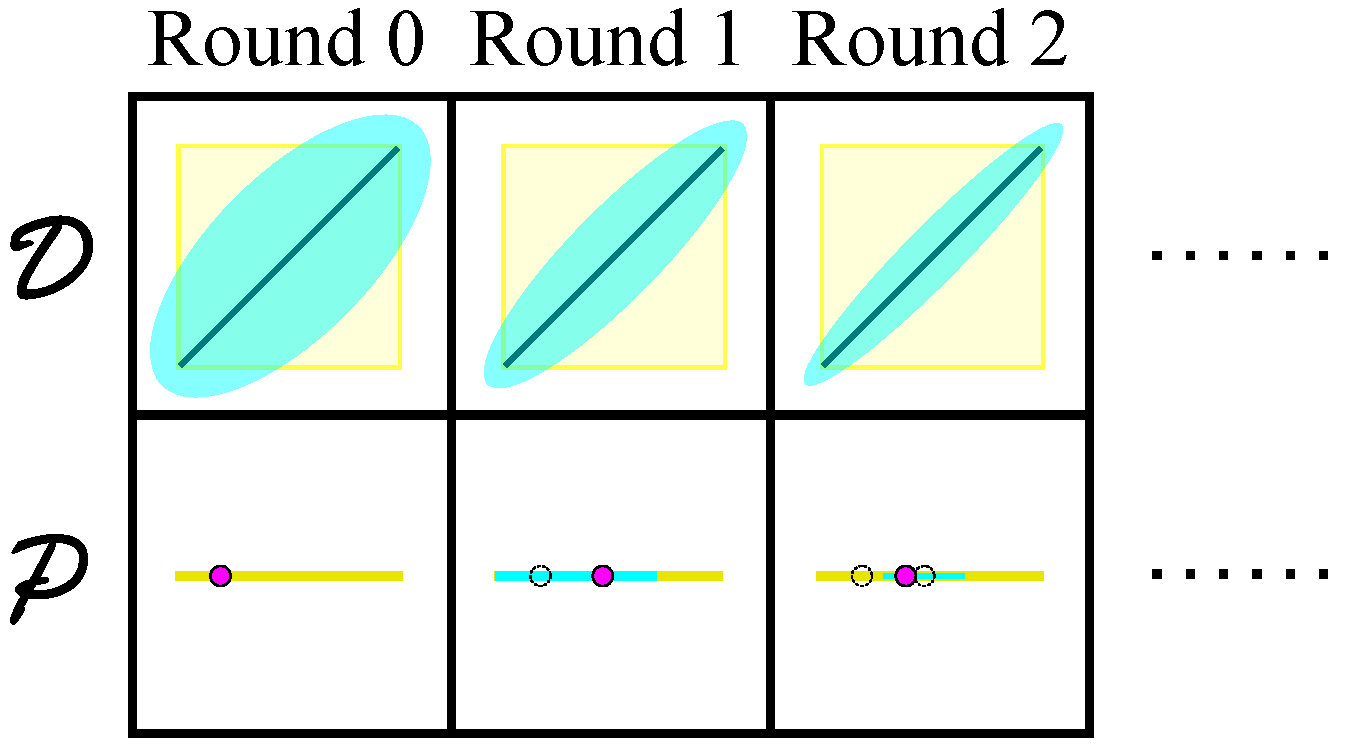
\includegraphics[width=0.6\linewidth]{proximalGamePrime.pdf}
    \end{figure}

  $\pl D$ wins the game if the points chosen by $\pl P$ converge.
  Otherwise, $\pl P$ wins.
  \end{game}
\end{frame}

\subsection{Motivation}

\begin{frame}
  If $\pl D\win \bellAbsConGame{X}$, then $X$ is called an
  \term{absolutely proximal space}.
  ``Absolutely proximal'' is a strengthening of ``proximal'' characterized
  by an easier game (for \(\pl D\)), but these games are equivalent for
  compact spaces.

  \vpause

  This game connects to a game of Gary Gruenhage: \cite{MR3239205}

  \begin{theorem}
    Every proximal space is a $W$-space. So
    $\pl D\win\bellAbsConGame{X} \Rightarrow \pl O\win\gruConGame{X}{x}$
    for all $x\in X$.
  \end{theorem}
\end{frame}

\begin{frame}
  Proximal spaces have strong preservation properties, as any
  closed subset or $\Sigma$-product of proximal spaces is proximal.

  \vpause

  Since any metrizable space is proximal, and
  any proximal space is collectionwise normal, Bell's game gives an elegant
  proof of the classic result of Rudin and Gulko:

  \begin{theorem}
    A $\Sigma$-product of metrizable spaces is collection-wise normal.
  \end{theorem}
\end{frame}

\begin{frame}
  Nyikos \cite{MR3288115} observed that
  \begin{proposition}
    Corson compact spaces are proximal.
  \end{proposition}
  and asked if the converse holds as well.

  \vpause

  With Gruenhage, I showed that the answer is yes: \cite{MR3227201}
  \begin{theorem}
    A compact space is Corson compact if and only if it is proximal.
  \end{theorem}
\end{frame}


\section{Topological proximal game}

\subsection{Uniform Spaces}

\begin{frame}
  Player $\pl D$ chooses \term{entourages} of the diagonal: elements of
  a \term{uniformity} inducing the topology of the space.

  \vpause

  A uniformity $\mb D$ on $X$ is a filter of subsets of $X^2$
  satisfying:
  \begin{itemize}
    \item $\bigcap \mb D = \Delta=\{\<x,x\>:x\in X\}$
    \item $D\in\mb D$ implies $D^{-1}=\{\<y,x\>:\<x,y\>\in D\}\in\mb D$
    \item for each $D\in\mb D$ there is $\frac{1}{2}D\in\mb D$ such that
          $\frac{1}{2}D\circ\frac{1}{2}D\subseteq D$
  \end{itemize}

  \vpause

  The topology induced by a uniformity is the smallest topology such that
  $D[x]=\{y:\<x,y\>\in D\}$ is a neighborhood of $x$ for each $D\in\mb D$.
\end{frame}

\subsection{Universal uniformity}

\begin{frame}
  Our goal is to obtain a purely topological characterization of the
  proximal property.

  \vpause

  As it turns out, the union of all uniformities inducing a topology is
  itself a uniformity inducing that topology, called the
  \term{fine} or \term{universal uniformity}.
  Furthermore, the proximal property is agnostic to which uniformity
  is chosen for the space's topology.

  \vpause

  If there's a winning strategy for $\pl D$ given any uniformity for
  the topology on $X$, then
  that strategy also works with the universal uniformity for $X$
  containing it.
  This reduces our goal to characterizing the entourages of the
  universal uniformity.
\end{frame}

\begin{frame}
  If you look in the right textbook \cite{MR2048350}, you'll
  find the answer:

  \begin{theorem}
    A neighborhood $U$ of the diagonal is a universal entourage if
    and only if there
    exist neighborhoods $U_n$ for $n<\omega$ where $U=U_0$ and
    $U_{n+1}\circ U_{n+1}\subseteq U_n$.
  \end{theorem}

  \pause

  As a bonus, for paracompact spaces, \textit{all} neighborhoods of
  the diagonal have this property (entourages may be converted to open
  covers and then star-refined).

  \vpause

  So we topologize Bell's game by simply saying an ``entourage''
  is any open symmetric neighborhood of the diagonal with the above property,
  and discard the need to consider a specific uniform structure.
\end{frame}


\section{Limited information strategies}

\subsection{Definitions}

\begin{frame}
  A \term{perfect information strategy} uses full information of the
  previous moves of the opponent. ($\pl A\win G$)

  \vpause
  A \term{$k$-tactical strategy} only uses the last $k$
  previous moves of the opponent. ($\pl A\ktactwin{k} G$)

  \vpause
  A \term{$k$-Markov strategy} only uses the last $k$
  previous moves of the opponent and the round number.
  ($\pl A\kmarkwin{k} G$)

  \vpause
  If omitted, assume $k=1$.
\end{frame}

\subsection{Lemmas and generalizations}

\begin{frame}\small
  Bell observed that a winning perfect information strategy may always
  be passed down to win in a closed subspace.

  \begin{proposition}
    If $\pl D\win\bellAbsConGame{X}$, then
    $\pl D\win\bellAbsConGame{H}$ for every closed subspace $H$ of $X$.
  \end{proposition}

  \pause

  This also holds for limited information strategies:

  \begin{proposition}
    If $\pl D\ktactwin{k}\bellAbsConGame{X}$, then
    $\pl D\ktactwin{k}\bellAbsConGame{H}$ for every closed subspace $H$ of $X$.
  \end{proposition}

  \begin{proposition}
    If $\pl D\kmarkwin{k}\bellAbsConGame{X}$, then
    $\pl D\kmarkwin{k}\bellAbsConGame{H}$ for every closed subspace $H$ of $X$.
  \end{proposition}
\end{frame}

\begin{frame}
  Bell's also showed that winning strategies
  are preserved for $\Sigma$-products.

  \begin{theorem}
    If $\pl D\win\bellAbsConGame{X_\alpha}$ for $\alpha<\kappa$, then
    $\pl D\win\bellAbsConGame{\sum_{\alpha<\kappa}X_\alpha}$.
  \end{theorem}

  \vpause

  Idea of proof: during round $n$, consider the first $n$ non-zero coordinates
  of the previous $n$ moves by $\pl P$ and use the winning strategies for
  those finite coordinates. Note that this uses the round number
  and perfect information of all previous moves.

\end{frame}

\begin{frame}
  If we allow ourselves the round number, we may at least handle countable
  products:

  \begin{theorem}
    If $\pl D\kmarkwin{k}\bellAbsConGame{X_i}$ for $i<\omega$,
    then $\pl D\kmarkwin{k}\bellAbsConGame{\prod_{i<\omega} X_i}$.
  \end{theorem}

  It seems likely that
  $\pl D\notmarkwin\bellAbsConGame{\sum_{\alpha<\omega_1} 2}$,
  but I don't have a proof. Whether
  $\pl D\kmarkwin{2}\bellAbsConGame{\sum_{\alpha<\omega_1} 2}$
  holds is less clear.
\end{frame}

\subsection{An application}

\begin{frame}
  Existence of a winning limited information strategy characterizes a
  stronger topological property than the existence of a winning perfect
  information strategy.

  \vpause

  As it turns out:

  \begin{theorem}
    A compact space $X$ is strongly Eberlein compact if and only if
    $\pl D\tactwin\bellAbsConGame{X}$.
  \end{theorem}
\end{frame}

\begin{frame}{Sketch of Proof}
  Easy direction:

  \begin{definition}
    Strong Eberlein compacts embed in $\sigmaProdTwo\kappa$ for
    some $\kappa$.
  \end{definition}

  \begin{lemma}
    $\pl D\tactwin\bellAbsConGame{\sigmaProdTwo\kappa}$.
  \end{lemma}
\end{frame}

\begin{frame}{Sketch of Proof (cont.)}
  Lemmas which give the other direction:

  \begin{lemma}[Gruenhage \cite{MR752278}]
    Scattered proximal compacts are strong Eberlein compact.
  \end{lemma}

  \begin{lemma}
    Non-scattered proximal compacts contain copies of the Cantor space
    $2^\omega$.
  \end{lemma}

  \begin{lemma}
    $\pl D\nottactwin\bellAbsConGame{2^\omega}$.
  \end{lemma}
\end{frame}

\begin{frame}
  A neat corollary:

  \pause

  \begin{itemize}
  \item For compact spaces, \(\pl O\win\gruConGame{X^2}{\Delta}\) if and only
  if \(\pl D\win\bellAbsConGame{X}\).
  \end{itemize}

  \pause

  but:

  \begin{itemize}
  \item Any metric space satisfies \(\pl O\tactwin\gruConGame{X^2}{\Delta}\),
  but for compact spaces, \(\pl D\tactwin\bellAbsConGame{X}\) implies
  \(X\) is scattered.
  \end{itemize}
\end{frame}





\section{Questions?}

\begin{frame}
  Any questions?
\end{frame}


\begin{frame}[allowframebreaks]
  \tiny
  \bibliographystyle{plain}
  \bibliography{../../bibliography}
\end{frame}


\end{document}


